%% ----------------------------------------------------------------
%% Thesis.tex -- MAIN FILE (the one that you compile with LaTeX)
%% ---------------------------------------------------------------- 

% Set up the document
\documentclass[a4paper, 11pt, oneside]{Thesis}  % Use the "Thesis" style, based on the ECS Thesis style by Steve Gunn
\graphicspath{{Figures/}}  % Location of the graphics files (set up for graphics to be in PDF format)
\usepackage[flushleft]{threeparttable}
\usepackage[acronym]{glossaries}
\usepackage{array}
\usepackage{multirow}
\usepackage{subcaption}
\usepackage{algorithm}
\usepackage{algpseudocode}
\usepackage{longtable}
\usepackage{tabularx}
% Include any extra LaTeX packages required
\usepackage[square, numbers, comma, sort&compress]{natbib}  % Use the "Natbib" style for the references in the Bibliography
\usepackage{verbatim}  % Needed for the "comment" environment to make LaTeX comments
\usepackage{vector}  % Allows "\bvec{}" and "\buvec{}" for "blackboard" style bold vectors in maths
\hypersetup{urlcolor=blue, colorlinks=true}  % Colours hyperlinks in blue, but this can be distracting if there are many links.
\newcommand{\NewPage}{\newpage\null\thispagestyle{empty}\newpage}
\makeglossaries
%% ----------------------------------------------------------------
\begin{document}
\frontmatter	  % Begin Roman style (i, ii, iii, iv...) page numbering

% Set up the Title Page

\title  {A Multi-UAV Simulator for User Data Analysis}
\authors  {\texorpdfstring
            {\href{}{V\'ictor Rodr\'iguez Fern\'andez}}
            {V\'ictor Rodr\'iguez Fern\'andez}
          }
\supervisor {\texorpdfstring
             {\href{}{David Camacho Fern\'andez}}
             {David Camacho Fern\'andez}
            }            
\addresses  {\groupname\\\deptname\\\univname}  % Do not change this here, instead these must be set in the "Thesis.cls" file, please look through it instead
\date       {\today}
\subject    {}
\keywords   {Unmanned Aircraft Vehicles, Simulator, Videogames, Behavior analysis}
\claves   {Sistemas A\'ereos no tripulados, Planificaci\'on de Misiones, Simulador, An\'alisis de comportamiento}

\maketitle
%% ----------------------------------------------------------------

\setstretch{1.3}  % It is better to have smaller font and larger line spacing than the other way round

% Define the page headers using the FancyHdr package and set up for one-sided printing
\fancyhead{}  % Clears all page headers and footers
\rhead{\thepage}  % Sets the right side header to show the page number
\lhead{}  % Clears the left side page header

\pagestyle{fancy}  % Finally, use the "fancy" page style to implement the FancyHdr headers

%\NewPage
%% ----------------------------------------------------------------
% Declaration Page required for the Thesis, your institution may give you a different text to place here
%\Declaration{
%
%\addtocontents{toc}{\vspace{1em}}  % Add a gap in the Contents, for aesthetics
%
%I, Victor Rodriguez Fernandez, declare that this thesis titled, A Multi-UAV Simulator for User Data Analysis, and the work presented in it are my own. I confirm that:
%
%\begin{itemize} 
%\item[\tiny{$\blacksquare$}] This work was done wholly or mainly while in candidature for a Master degree at this University.
% 
%\item[\tiny{$\blacksquare$}] Where any part of this thesis has previously been submitted for a degree or any other qualification at this University or any other institution, this has been clearly stated.
% 
%\item[\tiny{$\blacksquare$}] Where I have consulted the published work of others, this is always clearly attributed.
% 
%\item[\tiny{$\blacksquare$}] Where I have quoted from the work of others, the source is always given. With the exception of such quotations, this thesis is entirely my own work.
% 
%\item[\tiny{$\blacksquare$}] I have acknowledged all main sources of help.
% 
%\item[\tiny{$\blacksquare$}] Where the thesis is based on work done by myself jointly with others, I have made clear exactly what was done by others and what I have contributed myself.
%\\
%\end{itemize}
%
%
%{\large This work is supported by the Spanish Ministry of Science and Education under Project Code TIN2010-19872 and Savier Project (Airbus Defence \& Space, FUAM-076915).}
%
% 
% 
%Signed:\\
%\rule[1em]{25em}{0.5pt}  % This prints a line for the signature
% 
%Date:\\
%\rule[1em]{25em}{0.5pt}  % This prints a line to write the date
%}
%\clearpage  % Declaration ended, now start a new page

%% ----------------------------------------------------------------
% The "Funny Quote Page"
\NewPage
\pagestyle{empty}  % No headers or footers for the following pages

\null\vfill
% Now comes the "Funny Quote", written in italics
\textit{``Drones, drones everywhere..."}

\begin{flushright}
The Beards
\end{flushright}

\vfill\vfill\vfill\vfill\vfill\vfill\null
\clearpage  % Funny Quote page ended, start a new page
%% ----------------------------------------------------------------

% The Abstract Page
\NewPage
\glsdisablehyper
\addtotoc{Abstract}  % Add the "Abstract" page entry to the Contents
\begin{abstract}
\addtocontents{toc}{\vspace{1em}}  % Add a gap in the Contents, for aesthetics

\begin{small}
%Abstract en inglés
English Abstract
\end{small}

\end{abstract}

\clearpage  % Abstract ended, start a new page
%% ----------------------------------------------------------------

% Pagina Resumen
\NewPage
\glsdisablehyper
\addtotoc{Resumen}  % Add the "Abstract" page entry to the Contents
\begin{resumen}
\addtocontents{toc}{\vspace{1em}}  % Add a gap in the Contents, for aesthetics

\begin{small}
%Abstract en español
Spanish Abstract
\end{small}

\end{resumen}

\clearpage  % Abstract ended, start a new page
%% ----------------------------------------------------------------

\NewPage
\setstretch{1.3}  % Reset the line-spacing to 1.3 for body text (if it has changed)

% The Acknowledgements page, for thanking everyone
\acknowledgements{
\addtocontents{toc}{\vspace{1em}}  % Add a gap in the Contents, for aesthetics

Acknowledgements

}
\clearpage  % End of the Acknowledgements
\NewPage
%% ----------------------------------------------------------------

\pagestyle{fancy}  %The page style headers have been "empty" all this time, now use the "fancy" headers as defined before to bring them back


%% ----------------------------------------------------------------
\lhead{\emph{Contents}}  % Set the left side page header to "Contents"
\tableofcontents  % Write out the Table of Contents

%% ----------------------------------------------------------------
\lhead{\emph{List of Figures}}  % Set the left side page header to "List if Figures"
\listoffigures  % Write out the List of Figures

%% ----------------------------------------------------------------
\lhead{\emph{List of Tables}}  % Set the left side page header to "List of Tables"
\listoftables  % Write out the List of Tables
%% ----------------------------------------------------------------
\setstretch{1.5}  % Set the line spacing to 1.5, this makes the following tables easier to read
\clearpage  % Start a new page
\lhead{\emph{Abbreviations}}  % Set the left side page header to "Abbreviations"
\listofsymbols{ll}  % Include a list of Abbreviations (a table of two columns)
{
% \textbf{Acronym} & \textbf{W}hat (it) \textbf{S}tands \textbf{F}or \\

%ACRONIMOS
\newacronym{ai}{AI}{Artificial Intelligence}
\textbf{AI} & \textbf{A}rtificial \textbf{I}ntelligence  \\

\newacronym{bt}{BT}{Backtracking}
\textbf{BT} & \textbf{B}ack\textbf{T}racking \\

\newacronym{csop}{CSOP}{Constraint Satisfaction Optimization Problem}
\textbf{CSOP} & \textbf{C}onstraint \textbf{S}atisfaction \textbf{O}ptimization  \textbf{P}roblem \\

\newacronym{csp}{CSP}{Constraint Satisfaction Problem}
\textbf{CSP} & \textbf{C}onstraint \textbf{S}atisfaction \textbf{P}roblem \\

\newacronym{ga}{GA}{Genetic Algorithm}
\textbf{GA} & \textbf{G}enetic \textbf{A}lgorithm \\

\newacronym{gcs}{GCS}{Ground Control Station}
\textbf{GCS} & \textbf{G}round \textbf{C}ontrol \textbf{S}tation \\

\newacronym{hci}{HCI}{Human Computer Interface}
\textbf{HCI} & \textbf{H}uman \textbf{C}omputer \textbf{I}nterface \\

\newacronym{ia}{IA}{Interval Algebra}
\textbf{IA} & \textbf{I}nterval \textbf{A}lgebra \\

\newacronym{pof}{POF}{Pareto Optimal Frontier}
\textbf{POF} & \textbf{P}areto \textbf{O}ptimal \textbf{F}rontier  \\

\newacronym{tcsp}{TCSP}{Temporal Constraint Satisfaction Problem}
\textbf{TCSP} & \textbf{T}emporal \textbf{C}onstraint  \textbf{S}atisfaction \textbf{P}roblem \\

\newacronym{uas}{UAS}{Unmanned Aircraft System}
\textbf{UAS} & \textbf{U}nmanned \textbf{A}ircraft \textbf{S}ystem \\

\newacronym{uav}{UAV}{Unmanned Air Vehicle}
\textbf{UAV} & \textbf{U}nmanned \textbf{A}ir \textbf{V}ehicle \\

\newacronym{ums}{UMS}{UAV Mission Simulator}

\newacronym{uv}{UV}{Unmanned Vehicle}

\newacronym{us}{US}{Unmanned System}
}

%% ----------------------------------------------------------------
%\clearpage  % Start a new page
%\lhead{\emph{Physical Constants}}  % Set the left side page header to "Physical Constants"
%\listofconstants{lrcl}  % Include a list of Physical Constants (a four column table)
%{
%% Constant Name & Symbol & = & Constant Value (with units) \\
%Speed of Light & $c$ & $=$ & $2.997\ 924\ 58\times10^{8}\ \mbox{ms}^{-\mbox{s}}$ (exact)\\

%}

%% ----------------------------------------------------------------
%\clearpage  %Start a new page
%\lhead{\emph{Symbols}}  % Set the left side page header to "Symbols"
%\listofnomenclature{lll}  % Include a list of Symbols (a three column table)
%{
%% symbol & name & unit \\
%$a$ & distance & m \\
%$P$ & power & W (Js$^{-1}$) \\
%& & \\ % Gap to separate the Roman symbols from the Greek
%$\omega$ & angular frequency & rads$^{-1}$ \\
%}
%% ----------------------------------------------------------------
% End of the pre-able, contents and lists of things
% Begin the Dedication page

%\setstretch{1.3}  % Return the line spacing back to 1.3

%\pagestyle{empty}  % Page style needs to be empty for this page
%\dedicatory{Dedicated to my father. Your son is doing well.}

%\addtocontents{toc}{\vspace{2em}}  % Add a gap in the Contents, for aesthetics


%% ----------------------------------------------------------------
\mainmatter	  % Begin normal, numeric (1,2,3...) page numbering
\pagestyle{fancy}  % Return the page headers back to the "fancy" style

% Include the chapters of the thesis, as separate files
% Just uncomment the lines as you write the chapters
\glsresetall

% Chapter 1

\chapter{Introduction} % Write in your own chapter title
\label{Chapter1}
\lhead{Chapter 1. \emph{Introduction}} % Write in your own chapter title to set the page header


\section{Motivation}


\section{Objectives}

\section{Document structure}
 % Introduction

% Chapter 2

\chapter{Related Work} % Write in your own chapter title
\label{Chapter2}
\lhead{Chapter 2. \emph{Related Work}} % Write in your own chapter title to set the page header

The study of \glspl{uav} is wide and goes

In this chapter, we introduce a state of the art on \glspl{ums}, focusing on their main features, objectives, complexity and accessibility.

\section{UAV Simulators}
%Hablar de todo tipo de simuladores (Comerciales, no comerciales...)
Computer simulations, and their extension into videogames, of \glspl{us} are an emerging topic. There are at least three motivations for these type of simulators. One is the role of simulators in adoption of new technology, another is their potential for low cost training, and finally their utility in research. The four critera used to jugde the quality of any virtual simulator are defined in \cite{alexander2005gaming}:
\begin{enumerate}
\item \emph{Physical Fidelity}: It can be described as the extent to which the virtual environment emulates the real world. A simulator with high physical fidelity is able to render the environment with high resolution textures, shaders, lighting, reflection, and bump mapping. A low physical fidelity simulator uses 2D rendering and no sound is required.

\item \emph{Functional Fidelity}: The degree to which the simulation acts like the operational equipment in reacting to the tasks executed by the trainee. High functional fidelity is defined as the simulation of most of the forces acting on a vehicle and its actuators including gravity, drag, and accelerations from motors and collisions on specific elements of the vehicle. A low functional fidelity simulator does not simulate forces applied to the vehicle but only velocities or absolute position.

\item \emph{Ease of Development}: It is defined by how easy/difficult the simulator can be modified, and the available documentation from the author.

\item \emph{Cost}: For a simulator to be useful it must not be time consuming to install or run and accessible in terms of initial monetary cost for both the developer and end user. The simulator developed in this work is focused on maximizing this criteria.
\end{enumerate}

%Talk about the low cost UV simulators surveyed in craighead2007survey
\cite{craighead2007survey} surveys multiple \gls{us} simulators, both commercial and open-source, and provides a subjective rating of capabilities in terms of physical fidelity, functional fidelity, ease of use, and cost. For the purposes of this work, we focus only on those rated as "Low" in the Cost criteria. Table \ref{table:lowCostUVSimulators} summarizes the rating results of the aforementioned "Low cost" \gls{us} Simulators:

\begin{itemize}
\item \emph{FlightGear}: FlightGear \cite{flightGear} is a 3D open source simulator, very realistic and focused on simulating the flight of a single aircraft vehicle. It is available as a free download under GPL license. The entire source code is available for modification and is under constant development. The application runs on Windows, Mac, and Linux operating systems. It has been used for various academic projects. For example, Summers, et al. in \cite{summers2002determination} used FlightGear to simulate a \gls{uav} carrying environmental sensors and Cervin, et al. in \cite{cervin20043d} used FlightGear to create an interface for a real \gls{uav}.

\item \emph{Simbad}: Simbad \cite{simbad} is a Java 3d robot simulator for scientific and educational purposes. It is mainly dedicated to researchers/programmers who want a simple basis for studying Situated Artificial Intelligence, Machine Learning, and more generally AI algorithms, in the context of Autonomous Robotics and Autonomous Agents. It is not intended to provide a real world simulation and is kept voluntarily readable and simple.

\item \emph{SimRobot}: SimRobot \cite{simrobot} is a physics based robot simulator with a 3D OpenGL based display. Several sensor types are supported, including cameras, range sensors, touch 
sensors, and actuator state. It was used by the German team for the 2005 RoboCup competition \cite{laue2006simrobot}.
\end{itemize}

Analyzing the simulators detailed above, it is appreciable that the Functional Fidelity rating for all of them is not high, thus we cannot use them to easily analyze human control over them. Also, none of them focuses on the field of \glspl{uav} purely, but cover general unmanned robots or aircrafts instead. This is because at the time when these simulators were released, \glspl{uav} did not have as much importance as now.

%More recent work (focused on UAVs strictely)
Recently, the rapidly increasing interest in \glspl{uav} has caused that they are no longer part of a flight simulator or a type of robot in a general robot simulator. Small/micro UAVs have become applicable in civilian circumstances like remote sensing, mapping, traffic monitoring, search and rescue, etc. They are expendable, easy to be built and operated. Most of them can be operated by one to two people, or even be hand-carried and hand-launched \cite{roadmap2002roadmap,wu2004micro}. This has caused a large increase in the development of the so-called \emph{Autopilots}.

%Autopilots - Survey
\emph{Autopilots} are systems to guide the \glspl{uav} in flight with no assistance from human operators, consisting of both hardware and its supporting software. In \cite{chao2010autopilots}, both commercial and research autopilot systems for small \glspl{uav} are reviewed and discussed in detail. Since this work is not emphasized on hardware, the most remarkable autopilot from that survey, in terms of software development, is \emph{Paparazzi}.

%Paparazzi
Paparazzi \cite{brisset2006paparazzi} is an open-source project, very popular among researchers, highlighted by offering good flexibility and ease to modify the autopilot based on own requirements (High "Ease of development" rate, following the criteria of \cite{alexander2005gaming}). For the software, it can achieve waypoint tracking, auto-takeoff and landing, and altitude hold. Figure \ref{fig:paparazziGCS} shows how this software tries to imitate a real \gls{gcs}. A disadvantage of Paparazzi (and more generally, of all autopilots surveyed in \cite{chao2010autopilots}), is the lack of support for cooperative control functions, required for some large area tasks that need multiple \glspl{uav} to perform them.

\begin{figure}[hbt]
	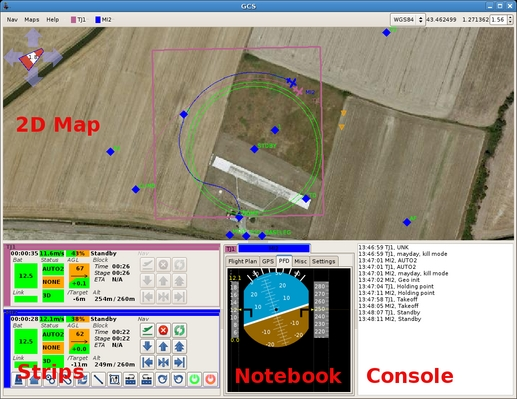
\includegraphics[width=\textwidth]{./Figures/PaparazziGCS.jpg}
	\centering
	\caption{Paparazzi GCS. The Paparazzi Ground Control Station is the heart of the system and the user's primary interaction interface.}
	\label{fig:paparazziGCS}
\end{figure}

%Multi UAV simulators and autopilots
The increasing demand and complexity of \gls{uav} applications has brought into focus several challenges associated with multiple \glspl{uav} \cite{bertuccelli2009real}. Although several researchers have done quite some experiments in this topic [28,29,27], few commercial autopilot systems have true multi-UAV functions built in.

%Barcelona simulator

%SARGE (Search And Rescue Game Environment)


%Low cost UV Simulators table
\begin{table}[hbt]	
\caption{A comparison of available Low-Cost Unmanned Vehicle Simulators.}
\label{table:lowCostUVSimulators}
\centering
\begin{tabularx}{\textwidth}{|X|X|X|X|X|}
\hline
\textbf{Simulator} & \textbf{Physical Fidelity} & \textbf{Functional Fidelity} & \textbf{Ease of Development} & \textbf{Cost}

\\ \hline
FlightGear & High & Medium & Medium & Low
\\ \hline
Simbad & Medium & Low & Medium & Low
\\ \hline
SimRobot & Medium & Low & Medium & Low 
\\ \hline
\end{tabularx}
\end{table}


%Especializarse en la situación de los simuladores Multi-UAV
\subsection{Multi-UAV Simulators}

%comentar los elementos gamers que suele haber en esta clase de simuladores
\subsection{Gamification in UAV Simulators}

\section{User Profile Analysis}
Computer simulation and video games are pedagogically proven techniques for training. Recent studies have shown that game-based learning have the potential to improve the transfer of skills over classroom-based activities \cite{alexander2005gaming,aitkin2004playing,green2003action}.

\subsection{Behavior Analysis in Video games}
\NewPage % Related Work

%% Chapter 3

\chapter{Architecture Model for UAV Mission Planning} % Write in your own chapter title
\label{Chapter3}
\lhead{Chapter 3. \emph{Architecture Model for UAV Mission Model}} % Write in your own chapter title to set the page header

\gls{uav} missions consists of a number $n$ of tasks performed by a team of $m$ \glspl{uav}. The main goal to solve the Misison Planning problem is to assign each task with an \gls{uav} that is able to perform it in a departure time sufficient to reach the task area in time. Note that the \gls{uav} could be parked at an airport or in flight after performing a previous task. %For this simple approach, we will despise the \gls{uav} fuel and time costs due to the takeoff and loiter during tasks development.
Figure \ref{fig:missionPlanning} shows an overview of the mission planning process.

\begin{figure}[h]
\centering
\includegraphics[width=0.6\textwidth]{./Figures/missionPlanning.png}
\caption{Mission Planning overview.}
\label{fig:missionPlanning}
\end{figure}

In this process, the Mission Planner receives a big amount of data about the environment, the available vehicles and its sensors and the mission for the purpose of using it for planning. The mission planner uses this information to compute the plans and then returns a set of tuples $<Task, Vehicle, Time>$ that specifies what tasks must do a \gls{uav} in a determinate moment.

Aiming to reproduce this functionality, we have developed a Mission Planning framework, that will be shown in next section.


\section{Framework Architecture}\label{architecture}
The architecture of the framework developed is shown in Figure \ref{fig:framework}. In this architecture, the Mission Planner, which is placed in the Mission Planning Module, uses a \gls{csp} solver, in this case Gecode \cite{SchulteEtAl2010}, to model and solve the \gls{tcsp} model that will be explained in section \ref{tcspmodel}. The planner receives the resource information (i.e. the information about the zones, sensors and \glspl{uav} involved in the mission), which is a static information stored in the system. On the other hand, the operator of the mission, through a \gls{hci}, provides the information about the mission (i.e. its tasks). After the execution of the Mission Planner, it returns a set of plans or solutions, which contain the tuples $<Task, Vehicle, Time>$ and some extra information about the estimated parameters of the mission, such as the fuel consumption, the speed of the vehicles, the total flight time, etc.


\begin{figure}[h]
\centering
\includegraphics[width=0.7\textwidth]{./Figures/architecture.png}
\caption{Mission Planning Framework Architecture.}
\label{fig:framework}
\end{figure}

The following sections will describe in detail the data model used in the Mission Planner and the \gls{tcsp} modelling of the mission planning problem.

\section{Mission Data Model}\label{datamodel}
The data model used in the Mission Planner can be divided in four components related to the Sensors (or Payloads), Zones, \glspl{uav} and Mission (or Tasks) information. The next subsections explain each one of these components in detail.


\subsection{Sensors}
Sensors or payloads are attached to vehicles and they permit developing the tasks of the mission, such as taking photos or tracking a zone. Figure \ref{fig:sensor} shows a UML data model of class sensor and its main subclasses.

\begin{figure}[h]
\centering
\includegraphics[width=0.7\textwidth]{./Figures/sensors.png}
\caption{Sensor UML Data Model.}
\label{fig:sensor}
\end{figure}

In this work, we have considered three different sensors:

\begin{itemize}

\item Camera Electro-Optical/Infra-red (EO/IR): This sensor allow the \gls{uav} to take photos. It has some internal features, such as the type of the camera, its zoom, resolution and its modes.

\item Radar: It allows to track the elements in a zone near the vehicle. Its main feature is the type of the radar (SAR, I-SAR or GMTI).

\item Communications Equipment: This equipment allows the \gls{uav} to communicate and send real-time pictures to the \gls{gcs}.

\end{itemize}


\subsection{Zones}\label{zones}
Zones or areas are used to represent the place where the tasks of the mission are developed. Figure \ref{fig:zone} shows a UML data model of class Zone and its associate classes.

\begin{figure}[h]
\centering
\includegraphics[width=0.7\textwidth]{./Figures/zones.png}
\caption{Zone UML Data Model.}
\label{fig:zone}
\end{figure}

\subsubsection{Coordinates}
The class \textit{Coordinates} is used to represent a geographic point. It is composed by its Longitude, Latitude and Altitude. In this work, the distance between two points (name them, $x_1 [long_1,lat_1,alt_1]$ and $x_2[long_2,lat_2,alt_2]$) is computed using the Haversine formula with the latitude and longitude:
\small
\begin{equation}
	d_{2D} (x_1,x_2) = 2r_{EARTH} \arcsin\sqrt{\sin^2(\frac{lat_2-lat_1}{2}) + \cos(lat_1) \cos(lat_2) \sin^2(\frac{long_2-long_1}{2})}
\end{equation}
\normalsize

and then the Euclidean distance with the resulting and the altitude

\begin{equation}
	d_{3D} (x_1,x_2) = \sqrt{d_{2D}^2(x_1,x_2)+(alt_2-alt_1)^2}.
\end{equation}

Besides, the bearing between two points is computed as:
\small
\begin{equation}
	\theta_{12}=arctan2(\sin(long_2-long_1) \cos(lat_2), \cos(lat_1) \sin(lat_2) - \sin(lat_1) \cos(lat_2) \cos(long_2-long_1))
\end{equation}
\normalsize


\subsubsection{Line}
On the other hand, the class \textit{Line}, which extends from class \textit{Segment}, is composed by two points. The 2D distance from a line (name it, $l_1$ with points $x_1$ and $x_2$) to a external point (name it, $x_3[long_3,lat_3,alt_3]$) is computed using the cross-track distance:

\begin{equation}
	d_{2D} (l_1,x_3)= \arcsin(\sin({\delta}_{13}) \sin ({\theta}_{13}-{\theta}_{12})) r_{EARTH}
\end{equation}

where ${\delta}_{13}$ is the distance between the point and the first vertex of the line,  ${\theta}_{13}$  is the starting bearing between the first vertex of the line and the point and ${\theta}_{12}$ is the starting bearing between the first vertex and the second vertex of the line.

Then, the 3D distance is computed using Euclidean distance with the 2D distance and the altitude difference of the point to the closest point in the line:

\begin{equation}
	d_{3D} (l_1,x_3)= \sqrt{d_{2D}^2(l_1,x_3)+(alt_{closest}-alt_3)^2}.
\end{equation}

The altitude of the closest point is directly known from:

\begin{equation}
	alt_{closest}=alt_1 + (alt_2-alt_1)*\frac{\arccos(\frac{\cos({\delta}_{13}/r_{EARTH})}{\cos(d_{2D}(l_1,x_3)/r_{EARTH})})r_{EARTH}}{{\delta}_{12}}.
\end{equation}


\subsubsection{Zone}
The class \textit{Zone} represents an area where a task is developed. An zone is composed by

\begin{itemize}

\item Several segments. As the only type of segment implemented is the line, a zone is a polygon (or a polygonal prism).

\item An altitude window $[h_{min},h_{max}]$ defined by the minimum and maximum altitude.

\item A flag indicating whether the zone is restricted or not. 

\end{itemize}

The class Zone determines whether a zone is closed or not if all the points of every segment is repeated at least twice. The position of a point respect to a zone is determined using the winding number algorithm:

\begin{algorithm}
\caption{Calculate the position of a point respect to a zone.}
\label{} 
\begin{algorithmic}
\State $cumulated = 0$
\For {each segment of the zone}
	\If {$(initLong - pointLong) \cdot (pointLong - endLong) \geq 0$ AND $(initLat - pointLat) \cdot (pointLat - endLat) \geq 0$ AND $(pointLongitude - initLongitude) \cdot (endLatitude - initLat) = (pointLat - initLat) \cdot (endLong - initLong))$}
		\If {$pointAlt < minAlt$ OR $pointAlt > maxAlt$}
			\State \Return OUTSIDE
		\EndIf
		\State \Return BOUND
	\EndIf
	\State $angle = point.endBearing(init) – point.endBearing(end)$
	\If {$angle \geq PI$} 
		\State $angle -= 2*PI$
	\Else
		\If {$angle \leq -PI$}
			\State $angle += 2*PI$
		\EndIf
	\EndIf
	\State $cumulated += angle$
\EndFor
\If {$cumulated/PI = 0$ OR $pointAlt < minAlt$ OR $pointAlt > maxAlt$}
	\State \Return OUTSIDE
\Else
	\State \Return INSIDE
\EndIf
\end{algorithmic}
\end{algorithm}

Finally, the distance from a point to a zone is computed as the minimum distance to any of the segments of the zone.


\subsection{\glspl{uav}}
A mission counts with a number $m$ of available \glspl{uav} for its development. Each \gls{uav} (named it, \gls{uav} $k$) has some specific characteristics:

\begin{itemize}

\item Position and fuel at the beginning of the mission.
\item Fuel consumption rate
\item The maximum reachable speed $v_{k,max}$ 
\item The minimum cruise speed $v_{k,min}$
\item Maximum and minimum flight altitude $[h_{min},h_{max}]$
\item Permission to go to restricted zones
\item Available sensors $P_k$ (cameras, radars, communication equipments, \ldots)

\end{itemize}

Moreover, in each point in time, each \gls{uav} is positioned at some specific \textit{coordinates}, flies at some specific \textit{cruise speed} $v_{k \to i}$ and is filled with a specific amount of \textit{fuel}.

Figure \ref{fig:uav} shows the class UAV and its attributes. Some additional attributes, such as the maxFlightTime and the withinRange are not consider in the modelling, but they have been added for future works.

\begin{figure}[h]
\centering
\includegraphics[width=0.7\textwidth]{./Figures/uav.png}
\caption{UAV UML Data Model.}
\label{fig:uav}
\end{figure}

\subsection{Tasks}
A mission consists of a set of $n$ tasks to be performed. A task consists of performing an action in a specific zone, such as exploring the area or search for an object. Therefore, each task (name it, task $i$) consist of:

\begin{itemize}

\item An action, which can be carried out thanks to the sensors or payloads $P_i$ belonging to a particular \gls{uav}. Table \ref{table:taskActions} shows the relation between actions and sensor needs.

\begin{table}[h]
\caption{Different task actions considered}
\label{table:taskActions}
\centering
\begin{tabular}{|c|c|c|}
\hline
Action ID & Action & Sensors Needed\\
\noalign{\hrule height 2pt}
A0 & Taking pictures of a zone & \begin{minipage}{2.5in}
    \vskip 4pt
    \begin{itemize}
    	\item Camera EO/IR
    \end{itemize}
    \vskip 4pt
\end{minipage} \\
\hline
A1 & Taking real-time pictures of a zone & \begin{minipage}{2.5in}
    \vskip 4pt
    \begin{itemize}
    	\item Camera EO/IR
    	\item Communications Equipment
    \end{itemize}
    \vskip 4pt
\end{minipage} \\
\hline
A2 & Tracking a zone & \begin{minipage}{2.5in}
    \vskip 4pt
    \begin{itemize}
    	\item Radar SAR
    \end{itemize}
    \vskip 4pt
\end{minipage} \\
\hline
\end{tabular}
\end{table}


\item Geographic area with altitude window $[h_{min},h_{max}]$, which could be restricted.

\item Time interval with duration $\tau_i$ and end time $t_i$

\item Mean speed $\bar{v_i}$ at performing the task 

\end{itemize}

Figure \ref{fig:task} shows the class \textit{Task} and its attributes.

\begin{figure}[h]
\centering
\includegraphics[width=0.7\textwidth]{./Figures/task.png}
\caption{Task UML Data Model.}
\label{fig:task}
\end{figure}


\section{TCSP Mission Modelling}\label{tcspmodel}

Nowadays there are several functionally \gls{csp} solvers developed. Our purpose is to use one of these already developed solvers to model and solve our Mission Planning problem.

For this purpose, different \gls{csp} solver technologies have been studied (see Appendix \ref{AppendixA}) in order to choose the better one to be improved, not only the fastest but the most suitable to our aim.

From this study, Gecode \cite{SchulteEtAl2010} has been selected as the best tool for \gls{csp} solving in terms of efficiency. This tool will be used in the following section to model the mission planning problem.

\subsection{TCSP Modelling using Gecode}
One of the main advantages of using Gecode for \gls{tcsp} modelling is that, in its most recent versions, it provides float variables, which can be used for defining all the real variables of the problem: times, speeds, distances, \ldots These float variables and the constraints involving them are internally solved through Allen's \gls{ia} (see Chapter \ref{tcsp_rw}).

Now, the problem domain is modelled as a \gls{tcsp}. The main variables are the \textit{tasks} and their values will be the \textit{\glspl{uav}} that perform each task and their respective \textit{departure times}. Moreover, there are some additional variables: the cruise speed to reach the area of the task $v_{k \to i}$, the fuel cost, the distance travelled for each task; which can be deduced from tasks assignment and \gls{uav} characteristics.

Figure \ref{fig:assignment} shows an assignment of a \gls{uav} $k$ to a task $i$. In this representation, it must be considered that:

	\begin{figure}[h]
		\includegraphics[width=1\textwidth]{./Figures/taskExample.png}
		\centering
		\caption{Scenario for performance of task $i$ by \gls{uav} $k$.}
		\label{fig:assignment}
	\end{figure}

\begin{itemize}

\item The vehicle is positioned at $pos_{k,i}$ at departure time $t_{d_i}$

\item The distance travelled to reach the task area in time $d_{k \to i}$, is computed using the formulas from section \ref{zones}:
\begin{equation}
	d_{k \to i} = i.area.distance(pos_{k,i})
\end{equation}

\item The flight time of the vehicle is
\begin{equation}\label{eq:flightTime}
	{flightTime}_i= \frac{d_{k \to i}}{v_{k \to i}} + \tau_i
\end{equation}

\item The fuel consumed by the vehicle is
\begin{equation}\label{eq:fuelConsume}
	f_i=k.fuelConsume * (d_{k \to i} + \tau_i \bar{v_i})
\end{equation}

\end{itemize}

The main constraints defined in this model are as follows:

\begin{enumerate}

\item Temporal constraints assuring a \gls{uav} does not perform two tasks at the same time. Let $k$ be a \gls{uav} that executes two tasks $i$ and $j$, where $i$ takes place before $j$, then $t_i$ must precede the departure time $t_{d_j}$ (see Figure \ref{fig:assignment2}):

\begin{equation}\label{eq:temporalConstraint}
  t_i \leqslant t_{d_j} = t_j - {flightTime}_i
\end{equation}

	\begin{figure}[!h]
		\includegraphics[width=1\textwidth]{./Figures/taskExample2.png}
		\centering
		\caption{Scenario for performance of tasks $i$ and $j$ by \gls{uav} $k$.}
		\label{fig:assignment2}
	\end{figure}

\item Logical constraints:

\begin{enumerate}

\item Speed window constraints: the mean speed necessary to perform the task $i$, $\bar{v_i}$, must be contained in the speed window $v_{k,max}$ and $v_{k,min}$:

\begin{equation}
  v_{k,min} \leq \bar{v_i} \leq v_{k,max}
\end{equation}

\item Altitude window constraints: a UAV $k$, with an altitude window $k_{h_{max}}$ and $k_{h_{min}}$, performing a task $i$ developed in an area with an altitude window $h_{max}$ and $h_{min}$, must obey:

\begin{align}
  k.h_{max} \geq i.area.h_{max} \\
  k.h_{min} \leq i.area.h_{min}
\end{align}

\item Zone permission constraints: another constraint is the implication that a restricted area has in the tasks to perform. Just UAVs with permissions in those areas shall perform the tasks.

\end{enumerate}

\item Resource constraints:

\begin{enumerate}

\item Sensor constraints: another constraint is whether a UAV carries the corresponding sensor to perform a task. Let $P_k$ denote the sensors available for UAV $k$ and $P_i$ the sensors needed for the task $i$ (performed by $k$), then:

\begin{equation}
  P_i \subseteq P_k,
\end{equation}

\item Fuel constraints: finally, we must constraint the fuel cost for each UAV. The fuel cost for a UAV $k$ performing a task $i$ is

\begin{equation}\label{eq:fuel}
	f_i=k.fuelConsumeRate * (d_{k \to i} + \tau_i \bar{v_i})
\end{equation}

So the following inequality must be obeyed:

\begin{equation}
  \sum_{i \in T_k} f_i \leqslant k.fuel
\end{equation}

\end{enumerate}

\end{enumerate}

To compute the distance (needed for the compute of flight time, see Equation \ref{eq:flightTime}), it is necessary to know where the vehicle is located before the start of the task, i.e. its position $pos_{k,i}$. Therefore, we have created a $m \times n$ matrix of tasks to \gls{uav} position. This matrix is initialized with every row, i.e. the positions of a specific vehicle, to the initial position of that vehicle. Each time a task assignment is considered in the constraint propagation process, this matrix is updated with the computed position of each vehicle at the end of the task.

All the aforementioned variables and constraints have been computed in Gecode to represent the Mission Planning Model. In following chapters, it will be shown how to solve this model with some methods provided by the solver.


\subsection{Optimization Function and Constraint Optimization Problem}\label{optimization}
As in many real-life applications, we just want to find some good solutions, what can be achieved considering a \gls{csop}. In order to apply a method for solving \gls{csop}, a new optimization function has been designed. This new function is looking to optimize (minimize) 3 objectives:

\begin{itemize}
	\item The total fuel consumed, computed as the sum of the fuel consumptions for each task using equation \ref{eq:fuelConsume}.
	
	\item The number of \glspl{uav} used in the mission. A mission performed with a lower number of vehicles is usually better because the remaining vehicles can perform other missions at the same time.
	
	\item The total flight time,  which is computed as the sum of the flight times for each task using equation \ref{eq:flightTime}.
\end{itemize}

As Gecode does not provide a method for computing the \gls{pof}, our model uses weights to map these three objectives into a single cost function, as the similar approach \gls{wcop} \cite{TorrensEtAl02}. This function is computed as the sum of percentage values of these three objectives, as shown in Equation \ref{eq:OptimizationFunction}. In this sense, in the second experimental phase, a comparative assessment of weights for finding feasible solutions of the problem will be carried out.

\begin{align}\label{eq:OptimizationFunction}
  f_{cost}(i) = K_{F}\frac{Fuel(i)}{\max_j{Fuel(j)}} &+ K_{U}\frac{N^{\circ}UAVs(i)}{\max_j{N^{\circ}UAVs(j)}} + K_{T}\frac{Flight Time(i)}{\max_j{Flight Time(j)}}\nonumber \\[1em]
  & K_{F},K_{U},K_{T}\in[0,1],\qquad K_{F}+K_{U}+K_{T}=1
\end{align} % Architecture

%% Chapter 4

\chapter{Experimental Setup} % Write in your own chapter title
\label{Chapter4}
\lhead{Chapter 4. \emph{Experimental Setup}} % Write in your own chapter title to set the page header

Since the Mission Planning problem is so complex and recent in the state of the art, there does not exist datasets or benchmarks available. For this reason, some simple datasets have been developed.

In the following sections, we explain the implemented datasets for missions (including the topology of the mission scenario) and teams of \glspl{uav}, and the different schemas considered according to the temporal preferences between tasks.

\section{Missions datasets}
There has been designed 10 missions, each one composed by an increasing number of tasks from 1 to 10, i.e the first mission has one task; the second, two tasks; and so on. Table \ref{table:missions} shows the 10 considered tasks, where the first mission will execute task with ID T1; the second will execute tasks with IDs T1 and T2; and so on. This table shows the duration of the tasks instead of the start and end times. These times will be fixed on the experimental phase depending on the number of dependencies between the tasks. The action IDs come from Table \ref{table:taskActions}.

\begin{table}[h]
\caption{\gls{uas} mission with 10 tasks}
\label{table:missions}
\centering
\begin{tabular}{|c|c|c|c|c|c|}
\hline
Task ID & Action ID & Duration(min) & \begin{minipage}{1in}
    \vskip 4pt
    \centering
    Zone altitude\\
    window (km)
    \vskip 4pt
\end{minipage} & \begin{minipage}{1in}
    \vskip 4pt
    \centering
    Mean speed\\
    (km/h)
    \vskip 4pt
\end{minipage} & \begin{minipage}{1in}
    \vskip 4pt
    \centering
    Restricted\\
    zone?
    \vskip 4pt
\end{minipage}\\
\noalign{\hrule height 2pt}
T1 & A0 & 25 & {$[1.5-5]$} & 100 & NO \\
\hline
T2 & A2 &  20 & {$[1.5-5]$} & 100 & NO \\
\hline
T3 & A1 & 30 & {$[2.5-6.15]$} & 100 & YES \\
\hline
T4 & A0 & 25 & {$[0.5-3.75]$} & 100 & NO \\
\hline
T5 & A2 & 35 & {$[0.5-3.75]$} & 100 & NO \\
\hline
T6 & A1 & 30 & {$[3.85-5]$} & 100 & NO \\
\hline
T7 & A1 & 25 & {$[3.85-5]$} & 100 & NO \\
\hline
T8 & A1 &  12 & {$[1.5-5]$} & 100 & NO \\
\hline
T9 & A0 & 20 & {$[1.5-5]$} & 100 & NO \\
\hline
T10 & A2 & 25 & {$[2.5-6.15]$} & 100 & YES \\
\hline
\end{tabular}
\end{table}

In this approach, we consider the simple topology specified in Figure \ref{fig:topology}, where coloured areas represent the areas where tasks are performed and helicopters represent the airports where \glspl{uav} are situated at the beginning of the mission. In this scenario, there are four areas and four airports.

	\begin{figure}[!h]
		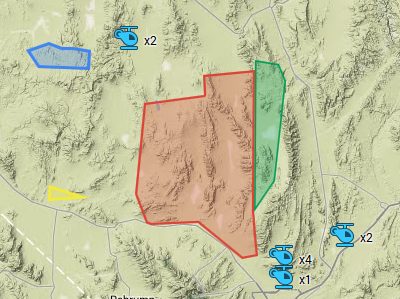
\includegraphics[width=0.8\textwidth]{./Figures/topology.png}
		\centering
		\caption{Topology of the scenario where missions are performed.}
		\label{fig:topology}
	\end{figure}


\section{\glspl{uav} datasets}
Different scenarios for solving the missions have been prepared with an increasing number of \glspl{uav} able to perform the tasks. The tasks contain several constraints, so when the number of tasks is very high, a high number of \glspl{uav} is also needed, mainly because of the fuel constraints. There has been considered groups of 1 to 9 vehicles available to perform the tasks (see Table \ref{table:uavs}). For a scenario with 1 vehicle, we use \gls{uav} with ID U1; for a scenario with 2 vehicles, \glspl{uav} with IDs U1 and U2; and so on.

\begin{table}[h]
\caption{Team of 9 available \glspl{uav}}
\label{table:uavs}
\centering
\begin{scriptsize}
\begin{tabular}{|c|c|c|c|c|c|c|}
\hline
\begin{minipage}{0.2in}
    \vskip 4pt
    \centering
    \gls{uav}\\
    ID
    \vskip 4pt
\end{minipage} & \begin{minipage}{0.7in}
    \vskip 4pt
    \centering
    Cruise speed\\
    window (km/h)
    \vskip 4pt
\end{minipage} & \begin{minipage}{0.6in}
    \vskip 4pt
    \centering
    Altitude\\
    window (km)
    \vskip 4pt
\end{minipage} & \begin{minipage}{0.7in}
    \vskip 4pt
    \centering
    Restricted zone\\
    permission
    \vskip 4pt
\end{minipage} & \begin{minipage}{0.5in}
    \vskip 4pt
    \centering
    Fuel consume\\
    (L/km)
    \vskip 4pt
\end{minipage} & \begin{minipage}{0.4in}
    \vskip 4pt
    \centering
    Initial\\
    Fuel (L)
    \vskip 4pt
\end{minipage} & Sensors Available \\
\noalign{\hrule height 2pt}
U1 & {$[90-110]$} & {$[0.3-6.5]$} & YES & 0.159 & 97.52 & \begin{minipage}{2in}
    \vskip 4pt
    \begin{itemize}
    	\item Camera EO/IR
    	\item Radar SAR
    	\item Communications Equipment
    \end{itemize}
    \vskip 4pt
\end{minipage} \\
\hline
U2 & {$[90-110]$} & {$[0.3-6]$} & NO & 0.159 & 58.48 & \begin{minipage}{2in}
    \vskip 4pt
    \begin{itemize}
    	\item Camera EO/IR
    \end{itemize}
    \vskip 4pt
\end{minipage} \\
\hline
U3 & {$[110-190]$} & {$[0.8-10]$} & YES & 0.2 & 140.23 & \begin{minipage}{2in}
    \vskip 4pt
    \begin{itemize}
    	\item Camera EO/IR
    	\item Radar SAR
    \end{itemize}
    \vskip 4pt
\end{minipage} \\
\hline
U4 & {$[90-110]$} & {$[0.3-6]$} & YES & 0.159 & 47.12 & \begin{minipage}{2in}
    \vskip 4pt
    \begin{itemize}
    	\item Camera EO/IR
    \end{itemize}
    \vskip 4pt
\end{minipage} \\
\hline
U5 & {$[90-110]$} & {$[0.3-6]$} & NO & 0.159 & 101.48 & \begin{minipage}{2in}
    \vskip 4pt
    \begin{itemize}
    	\item Camera EO/IR
    	\item Radar SAR
    	\item Communications Equipment
    \end{itemize}
    \vskip 4pt
\end{minipage} \\
\hline
U6 & {$[90-110]$} & {$[0.3-6]$} & NO & 0.159 & 101.37 & \begin{minipage}{2in}
    \vskip 4pt
    \begin{itemize}
    	\item Camera EO/IR
    	\item Radar SAR
    	\item Communications Equipment
    \end{itemize}
    \vskip 4pt
\end{minipage} \\
\hline
U7 & {$[90-110]$} & {$[0.3-6]$} & NO & 0.159 & 58.15 & \begin{minipage}{2in}
    \vskip 4pt
    \begin{itemize}
    	\item Camera EO/IR
    \end{itemize}
    \vskip 4pt
\end{minipage} \\
\hline
U8 & {$[110-190]$} & {$[0.8-10]$} & YES & 0.2 & 140.23 & \begin{minipage}{2in}
    \vskip 4pt
    \begin{itemize}
    	\item Camera EO/IR
    	\item Radar SAR
    \end{itemize}
    \vskip 4pt
\end{minipage} \\
\hline
U9 & {$[90-110]$} & {$[0.3-6]$} & YES & 0.159 & 47.12 & \begin{minipage}{2in}
    \vskip 4pt
    \begin{itemize}
    	\item Camera EO/IR
    \end{itemize}
    \vskip 4pt
\end{minipage} \\
\hline
\end{tabular}
\end{scriptsize}
\end{table}


\section{Temporal schemas}\label{temporalschemas}
Three scenarios have been generated with different temporal schemas based on the time dependencies between the tasks. Figure \ref{fig:tempoNoDep} shows an scenario with no time dependencies between tasks, i.e. the tasks do not collide in time. Figure \ref{fig:tempo1Dep} shows an scenario where each task collides in time with the previous task, i.e. there are $n-1$ temporal dependencies, being $n$ the number of tasks. Finally, when each task collides in time with the two previous tasks, i.e. there are $2(n-1)-1$ temporal dependencies, we have the scenario shown in Figure \ref{fig:tempo2Dep}.

	\begin{figure}[!h]
	\centering
		\begin{subfigure}[b]{0.9\textwidth}
			\includegraphics[width=\textwidth]{./Figures/tempoNoDep.png}
			\centering
			\caption{No dependencies}
			\label{fig:tempoNoDep}
		\end{subfigure}
		\begin{subfigure}[b]{0.9\textwidth}
			\includegraphics[width=\textwidth]{./Figures/tempo1Dep.png}
			\centering
			\caption{Dependency of each task with the previous task.}
			\label{fig:tempo1Dep}
		\end{subfigure}
		\begin{subfigure}[b]{0.9\textwidth}
			\includegraphics[width=\textwidth]{./Figures/tempo2Dep.png}
			\centering
			\caption{Dependency of each task with the two previous tasks.}
			\label{fig:tempo2Dep}
		\end{subfigure}
		\caption{Three schemas of the scenarios based on the number of temporal dependencies between the tasks.}
		\label{fig:tempo}
	\end{figure}
	
These schemas will be compared in the experimental phase (see Chapter \ref{Chapter5}) in order to observe the scalability of the problem as the number of temporal dependencies increase. % Experimental Setup

%% Chapter 5

\chapter{Experimental Results} % Write in your own chapter title
\label{Chapter5}
\lhead{Chapter 5. \emph{Experimental Results }} % Write in your own chapter title to set the page header

\section{Experiment 1: Search of the Complete Space of solutions with Backtracking}\label{experiment1}

\gls{bt} search implemented by Gecode solver has been used to solve the missions explained in the previous section, analysing the runtime spent in the process. This search algorithm performs constraint propagation with different consistency levels depending on the type of the constraint. For all the developed constraints in our problem, domain (or node) consistency is applied.

Due to some fuel and flight time constraints, with only 2 or 3 \glspl{uav} there is no solution for a high number of tasks $(> 6)$, so the solver has been run in different scenarios with 4 to 7 vehicles to test the scalability of the problem.

In the following sections, the scalability of the runtime and number of solutions obtained is studied based on the three different schemas from section \ref{temporalschemas}. First each schema is tested individually, and finally the three are compared between them.

\subsection{Study with temporally independent tasks}
Figures \ref{fig:noDependenciesSolutions} and \ref{fig:noDependenciesRuntime} shows the number of solutions and runtime obtained when the tasks do not collide in time (see Figure \ref{fig:tempoNoDep}). As we can see, the growth of the number of solutions is nearly exponential as the number of tasks increase. Indeed, the exponentiality is higher and more appreciable as the number of \glspl{uav} increase. For the runtime, the situation is similar, and the exponentiality growth is much higher. So it is clear that the scalability of the problem, as the number of variables increase, is exponential.

	%\begin{figure}[h]
		%\centering
		\begin{figure}[h]
			\centering
			\includegraphics[width=0.85\textwidth]{./Figures/noDependenciesSolutions}
			\caption{Number of solutions for missions with the No-Temporal Dependency Schema.}
			\label{fig:noDependenciesSolutions}
		\end{figure}
		\begin{figure}[h]
			\centering
			\includegraphics[width=0.85\textwidth]{./Figures/noDependenciesRuntime}
			\caption{Runtime for missions with the No-Temporal Dependency Schema}
			\label{fig:noDependenciesRuntime}
		\end{figure}
		%\caption{Results from the simulation of different missions with number of tasks from 1 to 10, where each task has no dependencies with any other, for groups of 4 to 7 UAVs.}
		%\label{fig:noDependencies}
	%\end{figure}

\subsection{Study with 1-temporal dependency tasks}
On the other hand, Figures \ref{fig:1DependencySolutions} and \ref{fig:1DependencyRuntime} shows what happens when each task collides in time with the previous task (see Figure \ref{fig:tempo1Dep}). As it can be seen, the growth is still pretty exponential for both the number of solutions and the runtime, but much smaller than with no dependencies. We also note that for less \glspl{uav} to perform the tasks, the exponentiality of the number of solutions disappears. This is because of the high number of constraints (increased with the new temporal constraints) that reduces the space search and, for a high number of tasks, makes the problem highly complex.

	%\begin{figure}[h]
		%\centering
		\begin{figure}[h]
			\centering
			\includegraphics[width=0.84\textwidth]{./Figures/1DependencySolutions}
			\caption{Number of solutions for mission with the 1-Temporal Dependency Schema.}
			\label{fig:1DependencySolutions}
		\end{figure}
		\begin{figure}[h]
			\centering
			\includegraphics[width=0.84\textwidth]{./Figures/1DependencyRuntime}
			\caption{Runtime for mission with the 1-Temporal Dependency Schema.}
			\label{fig:1DependencyRuntime}
		\end{figure}
		%\caption{Results from the simulation of different missions with number of tasks from 1 to 10, where each task collides in time with the previous, for groups of 4 to 7 UAVs.}
		%\label{fig:1Dependency}
	%\end{figure}

\subsection{Study with 2-temporal dependencies tasks}
When each task collides in time with the two previous tasks (see Figure \ref{fig:tempo2Dep}), the results in Figures \ref{fig:2DependenciesSolutions} and \ref{fig:2DependenciesRuntime}  show that the growth of the runtime is still exponential, but much smaller than in the two previous cases. On the other hand, the growth of the number of solutions has a more polynomial likely behaviour. We can notice how a great number of constraints affect the scalability of the solutions of the problem.
	
	%\begin{figure}[h]
		%\centering
		\begin{figure}[h]
			\centering
			\includegraphics[width=0.85\textwidth]{./Figures/2DependenciesSolutions}
			\caption{Number of solutions for missions with the 2-Temporal Dependencies Schema.}
			\label{fig:2DependenciesSolutions}
		\end{figure}
		\begin{figure}[h]
			\centering
			\includegraphics[width=0.85\textwidth]{./Figures/2DependenciesRuntime}
			\caption{Runtime for missions with the 2-Temporal Dependencies Schema.}
			\label{fig:2DependenciesRuntime}
		\end{figure}
		%\caption{Results from the simulation of different missions with number of tasks from 1 to 10, where each task collides in time with the two previous, for groups of 4 to 7 UAVs.}
		%\label{fig:2Dependencies}
	%\end{figure}

\subsection{Interdependency comparison}	
Finally, in Figures \ref{fig:interdependencySolutions} and \ref{fig:interdependencyRuntime} we can see for a group of 6 UAVs, a comparison of the results obtained according to the number of existing dependencies explained in the three previous experiments. We can see how the temporal constraints highly affect the space of solutions of the problem, but also the runtime necessary to find this new space of solutions.
	
	%\begin{figure}[h]
		%\centering
		\begin{figure}[h]
			\centering
			\includegraphics[width=0.85\textwidth]{./Figures/interdependencySolutions}
			\caption{Number of solutions for missions with the three temporal dependency schemas.}
			\label{fig:interdependencySolutions}
		\end{figure}
		\begin{figure}[h]
			\centering
			\includegraphics[width=0.85\textwidth]{./Figures/interdependencyRuntime}
			\caption{Runtime for missions with the three temporal dependency schemas.}
			\label{fig:interdependencyRuntime}
		\end{figure}
		%\caption{Comparison of the results from the simulations of different missions with number of tasks from 1 to 10 for a group of 6 UAVs; with no dependencies, one dependency with the previous task or dependencies with the two previous tasks between them.}
		%\label{fig:interdependency}
	%\end{figure}

On the other hand, we have computed the runtimes expended in these missions but with 9 \glspl{uav} (see table \ref{table:bt_runtime}), which will be compared to the runtimes expended at finding optimal solutions in the next experiment.

\begin{table}[h]
\caption{Runtime for missions with 1 to 10 tasks for a group of 9 \glspl{uav}, with the three temporal dependency schemas.}
\label{table:bt_runtime}
\centering
\begin{tabular}{|c||c|c|c|c|c|}
\hline
No. of tasks & \begin{minipage}{1.6in}
    \vskip 4pt
    \centering
    No Temp. Dep. Schema\\
    Runtime
    \vskip 6pt
\end{minipage} & \begin{minipage}{1.5in}
    \vskip 4pt
    \centering
    1 Temp. Dep. Schema\\
    Runtime
    \vskip 6pt
\end{minipage} & \begin{minipage}{1.5in}
    \vskip 4pt
    \centering
    2 Temp. Dep. Schema\\
    Runtime
    \vskip 6pt
\end{minipage}\\
\noalign{\hrule height 2pt}
1 task & 9.877ms & 69.072ms & 10.014ms \\
\hline
2 tasks & 182.606ms & 199.297ms & 173.222ms \\
\hline
3 tasks & 300.091ms & 253.523ms & 197.731ms \\
\hline
4 tasks & 3.002687s & 1.896258s & 1.517302s \\
\hline
5 tasks & 13.007988s & 7.490989s & 4.074907s \\
\hline
6 tasks & 51.789774s & 24.119561s & 11.333178s \\
\hline
7 tasks & 3m55s & 1m10s & 23.701752s \\
\hline
8 tasks & 18m55s & 3m51s & 47.584619s \\
\hline
9 tasks & 5h0m41s & 47m45s & 5m10s \\
\hline
10 tasks & 22h20m57s & 3h15m44s & 17m14s \\
\hline
\end{tabular}
\end{table}

\subsection{Conclusions}
In this experiment, we show that the model is easily computable using a known solver, and the entire space of solutions can be found provided that the mission is resolvable. From the obtained results, we have observed that the runtime necessary to search the entire space of solutions by \gls{bt} search is exponential as reported in literature. However, as the number of constraints increases (in this case the dependency constraints making tasks collide in time), the runtime decreases highly, but this scalability still resembles exponential. On the other hand, the number of solutions resembles exponential, but as the number of dependency constraints increases, the scalability loses its exponential behaviour and resembles more polynomial. This is due to the power of a dependency temporal constraint, which highly reduces the search space of solutions.

Although the runtime needed for exploring the space of solutions is exponential, we have seen that when there are too many constraints, as the number of tasks increase, there is a point where the resources of the available \glspl{uav} needed to supply all the tasks of the mission begin to decrease. In this situation, the number of solutions begins to decrease despite the increase of possible assignments due to a higher number of tasks.


\section{Experiment 2: Search of optimal solution with Branch \& Bound}\label{experiment2}

This second experiment treats with the scenario with a group of 9 \glspl{uav} to perform a mission of 10 tasks, and where each task collides in time with its two previous tasks, i.e. the 2-Temporal Dependency Schema.

Gecode provides a \gls{bb} search method for optimization problems, but does not automatically compute the \gls{pof}, so the cost function for the \gls{csop} will be the one explained in section \ref{optimization}.

This experiment starts comparing the different results obtained optimizing the different objectives individually and then take some of them to optimize altogether. Finally, the runtime results will be compared with the results from the previous \gls{bt} experiment in order to determine the order of the temporal gain from optimization.


\subsection{Individual Optimization}
\gls{bb} returns the best solution found based on the cost function used. So, firstly, an analysis of the optimal solution found considering as cost function each one of the objectives individually is carried out. It can be seen in Table \ref{table:solutionsIndividual}.

\begin{table}[h]
\caption{Objective values and runtime spent in the search of the optimal solution using cost functions considering individually each objective.}
\label{table:solutionsIndividual}
\centering
\begin{tabular}{|c|c|c|c||c|}
\hline
Cost function & Flight Time & No. of UAVs & Fuel & Runtime\\
\noalign{\hrule height 2pt}
100\% Fuel & 22h 8min 13s  & \textbf{4} & \textbf{269.561L} & 4min 9s \\
\hline
100\% No. of UAVs & 23h 22min 23s & \textbf{4} & 282.003L & \textbf{8.87s} \\
\hline
100\% Flight Time & \textbf{18h 0min 8s} & 8 & 284.875L & 7min 32s \\
\hline
\end{tabular}
\end{table}

It can be appreciated when considering cost function $100\%$ Flight Time that, besides the high runtime needed, the optimal solution found has a high number of \glspl{uav} and fuel consumption. This could be due to shorter flight times are obtained using \glspl{uav} that reach higher speeds but consuming more fuel, i.e. the flight time and the fuel consumption (or the number of UAVs too) have some kind of inverse relation. On the other hand, the number of \glspl{uav} and the fuel consumption are highly related.

Respect to the runtime, when considering the number of \glspl{uav} the optimization search finishes very soon, because this variable is computed directly from the assignments. The fuel consumption lasts a little more to be computed in each iteration, and the flight time is nearly the last variable being computed.

In the following experiment, we will try to optimize multiple variables at the same time. With this purpose, we will try to find a combination of weights that gets a optimal solution reducing the runtime as much as possible.


\subsection{Balanced cost function}
Attempting to optimize multiple objectives, there has been considered to use balanced cost function. Table \ref{table:solutionsBinary} shows solutions obtained when considering two objectives, while Table \ref{table:solutionsTernary} shows the ones when considering three objectives.

\begin{table}[h]
\caption{Objective values and runtime spent in the search of the optimal solution using binary balanced cost functions.}
\label{table:solutionsBinary}
\centering
\begin{tabular}{|c|c|c|c||c|}
\hline
Cost function & Flight Time & No. of UAVs & Fuel & Runtime\\
\noalign{\hrule height 2pt}
\begin{minipage}{1.5in}
50\% Fuel + \\
50\% No. of UAVs 
\end{minipage}  & 22h 8min 13s  & \textbf{4} & \textbf{269.561L} & \textbf{54.67s} \\
\hline
\begin{minipage}{1.5in}
50\% Fuel + \\
50\% Flight Time
\end{minipage} & \textbf{18h 29min 20s} & 7 & 279.353L & 8m11s \\
\hline
\begin{minipage}{1.5in}
50\% No. of UAVs + \\
50\% Flight Time 
\end{minipage}  & 19h 37min 58s & \textbf{4} & 278.436L & 2min 51s \\
\hline
\end{tabular}
\end{table}

\begin{table}[h]
\caption{Objective values and runtime spent in the search of the optimal solution using ternary balanced cost functions.}
\label{table:solutionsTernary}
\centering
\begin{tabular}{|c|c|c|c||c|}
\hline
Cost function & Flight Time & No. of UAVs & Fuel & Runtime\\
\noalign{\hrule height 2pt}
\begin{minipage}{2in}
33\% Fuel + 33\% No. of UAVs \\
 + 33\% Flight Time 
\end{minipage} & 20h 23min 33s  & 4 & 269.561L & 3m56s \\
\hline
\end{tabular}
\end{table}

Now it can be seen that combining weighted objectives reduce the runtime spent searching the solution compared to the previous individual optimization experiment in some cases. Specifically, we can see that combining the number of \glspl{uav} with the fuel consumption, gets an optimal solution for both variables. On the other hand, considering the flight time involves finding some suboptimal solutions for all the variables. In table \ref{table:solutionsTernary}, we can clearly see that the flight time is not optimized while the number of \glspl{uav} and the fuel consumption are.

Considering this aspect, we have decided to put the flight time variable aside and only consider the fuel consumption and the number of \glspl{uav}. So, in the next section, a simple experiment will be considered in which the fuel consumption and the number of \glspl{uav} are considered for a comparative assessment of optimization function weights.


\subsection{Optimizing the runtime with weighted cost functions}
Table \ref{table:solutionsFuelUAV} show the comparative assessment mentioned in the previously. For simplicity of the process, we have considered a weight step of $10\%$ between each instance tested.

\begin{table}[!h]
\caption{Objective values and runtime spent in the search of the optimal solution using cost functions considering fuel and number of UAVs with different percentages.}
\label{table:solutionsFuelUAV}
\centering
\begin{tabular}{|c|c|c|c||c|}
\hline
Cost function & Flight Time & No. of UAVs & Fuel & Runtime\\
\noalign{\hrule height 2pt}
100\% Fuel & 22h 8min 13s  & 4 & 269.561L & 4min 9s \\
\hline
90\% Fuel + 10\% No. of UAVs & 22h 8min 13s  & 4 & 269.561L & 3min 22s \\
\hline
80\% Fuel + 20\% No. of UAVs & 22h 8min 13s  & 4 & 269.561L & 2min 7s \\
\hline
70\% Fuel + 30\% No. of UAVs & 22h 8min 13s  & 4 & 269.561L & 1min 39s \\
\hline
60\% Fuel + 40\% No. of UAVs & 22h 8min 13s  & 4 & 269.561L & 1min 23s \\
\hline
50\% Fuel + 50\% No. of UAVs & 22h 8min 13s  & 4 & 269.561L & 54.67s \\
\hline
40\% Fuel + 60\% No. of UAVs & 22h 8min 13s  & 4 & 269.561L & 46.03s \\
\hline
30\% Fuel + 70\% No. of UAVs & 22h 8min 13s  & 4 & 269.561L & 35.02s \\
\hline
20\% Fuel + 80\% No. of UAVs & 22h 8min 13s  & 4 & 269.561L & \textbf{33.99s} \\
\hline
10\% Fuel + 90\% No. of UAVs & 22h 8min 13s  & 4 & 269.561L & 34.13s \\
\hline
100\% No. of UAVs & 23h 22min 23s & 4 & 282.003L & 8.87s \\
\hline
\end{tabular}
\end{table}

Analysing results shown in Table \ref{table:solutionsFuelUAV}, it can be appreciated that only considering the fuel consumption in a low percentage, an optimal solution both for the fuel and number of UAVs minimization is reached. Additionally, it is clearly appreciable that as the weight of the fuel consumption variable decreases, so it does the runtime spent in the search. Nevertheless, it can also be seen that the cost function $20\%$ fuel + $80\%$ No. of UAVs spends less runtime that the cost function $10\%$ fuel + $90\%$ No. of UAVs, breaking this linearity. This could be caused by some ``noise" in the execution of the program and the little difference of runtime between these two functions.

For this reason, it can be considered that a cost function of $10\%$ fuel + $90\%$ No. of UAVs is pretty good for searching feasible solutions in low runtime for this kind of problems.

Finally, in the next section, we will compare the runtime obtained with this cost function with the one obtained in the \gls{bt} experiment. In addition, we will compute the runtimes of this same problem with this cost function but considering the No-Temporal Dependencies Schema and the 1-Temporal Dependency Schema. Then, we will also compare these runtimes with the ones obtained in the \gls{bt} experiment.


\subsection{\gls{bt} vs \gls{bb}}
In this experiment, we have first calculated the runtime spent in the search of optimal solutions for the mission planning problem composed of 10 tasks and a group of 9 \glspl{uav} with the No-Temporal Dependencies Schema and 1-Temporal Dependency Schema (the 2-Temporal Dependencies Schema case was computed in the previous experiment) using \gls{bb} with the cost function $10\%$ fuel + $90\%$ No. of \glspl{uav}.

Then, the runtime spent in the search of feasible solutions and the runtime spent in the search of the entire space of solutions using \gls{bt} are compared in Table \ref{table:btvsbb}.

\begin{table}[h]
\caption{Runtime for missions with 10 tasks for a group of 9 \glspl{uav}, with the three temporal dependency schemas, using \gls{bt} and \gls{bb}.}
\label{table:btvsbb}
\centering
\begin{tabular}{|c||c|c|c|}
\hline
Algorithm & \begin{minipage}{1.3in}
\centering
No Dependencies \\
Schema Runtime
\end{minipage} & \begin{minipage}{1.3in}
\centering
1-Dependency \\
Schema Runtime
\end{minipage} & \begin{minipage}{1.3in}
\centering
2-Dependencies \\
Schema Runtime
\end{minipage} \\
\noalign{\hrule height 2pt}
BT & 22h20m57s & 3h15m44s & 17m14s \\
\hline
\begin{minipage}{1.5in}
\centering
B\&B (10\%  Fuel + \\
90\% No. of UAVs)
\end{minipage} & 11.33s & 26.74s & 34.13s \\
\hline
\end{tabular}
\end{table}

The time difference observed is high, as expected. A surprising fact is that, unlike it happened in \gls{bt} search, as the number of temporal constraints given by the temporal dependency schemas decrease, the runtime decreases. For instance, with the No-Temporal Dependency Schema, the runtime obtained for the \gls{bb} search is 11.33s; while the time obtained in the 2-Temporal Dependencies Schema is 34.13s. On the other hand, the runtime for \gls{bt} in the No-Temporal Dependency Schema is 22h 20min 57s, being higher than \gls{bb} in an order of $8 \cdot 10^3$; while in the 2-Temporal Dependencies Schema the runtime for \gls{bt} is 17min 14s, higher than \gls{bb} in an order of $30$ units.


\subsection{Conclusions}
In this second experiment, we have designed an optimization function to minimize four objectives: the fuel consumption, the number of \glspl{uav} used in the mission and the total flight time of all the \glspl{uav}. From the obtained results, we have observed that the flight time is the most difficult variable to compute, while the number of vehicles is the easiest.

Studying the solutions found by several cost functions with different weights for fuel and number of \glspl{uav}, we have observed how the runtime spent in the search decrease as the percentage of fuel decreases. Finally, we have compared the runtime from the \gls{bb} search obtained using the proposed weighted cost function $10\%$ fuel + $90\%$ No. of \glspl{uav} with the runtime obtained using \gls{bt}. As shown in the literature, this second is much higher; concretely we have observed that for this problem with the No-Temporal Dependency Schema it is $3 \cdot 10^3$ times higher. The most interesting fact observed is that the runtime spent in the \gls{bb} search decreases as the number of temporal constraints given by the temporal dependency schemas decreases.

It is important to remark that the results obtained are highly dependant on the proposed scenarios and on the topology of the areas the missions are developed in. So further works should consider different scenarios and topologies, so a more general conclusion would be obtained.

\NewPage % Experimental Results

%% Chapter 6

\chapter{Conclusions and Future Works} % Write in your own chapter title
\label{Chapter6}
\lhead{Chapter 6. \emph{Conclusions and Future Works }} % Write in your own chapter title to set the page header

\section{Conclusions}
In this work, we try to search feasible solutions for a \gls{uav} Mission Planning model based on \gls{tcsp}. The presented approach defines missions as a set of tasks to be performed by several \glspl{uav} with some capabilities. The problem is modelled using: (1) temporal constraints to assure that each \gls{uav} only performs one task at a time; (2) logical constraints such as the maximum and minimum altitude reachable or restricted zone permissions, and (3) resource constraints, such as the sensors and equipment needed or the fuel consumption, among others. This simple approach is quite close to real \gls{uav} missions, with less conditions treated.

Concretely, we have designed an optimization function to minimize three objectives: the fuel consumption, the number of \glspl{uav} used in the mission and the total flight time of all the \glspl{uav}.

We have shown that the model is easily computable using a known solver, i.e. Gecode, and both the entire space of solutions (using \gls{bt}) and the optimal solution (using \gls{bb}) can be found provided that the mission is resolvable.

From the obtained results, we have observed that the runtime necessary to search the entire space of solutions using \gls{bt} search is exponential, as reported in literature, but decreases as the number of constraints increase (because of the decrease of the number of possible solutions).

On a second experiment, we have shown that the \gls{wcop} approach is very useful to find a optimal solution, but not for computing the entire \gls{pof}. We have also observed that is very important to consider bigger weights in variables that are computed faster in order to improve the runtime. An interesting fact observed is that the runtime spent in the \gls{bb} search decreases as the number of temporal constraints given by the temporal dependency schemas decreases.


\section{Future works}
As future lines of work, this developed \gls{uav} Mission Planning model will be improved in order to consider a model as close as possible to real missions. We will consider the \gls{gcs} as a new scheduling part of the model, in order to decide the \gls{gcs} for each \gls{uav}. We will also consider refuelling tasks, which will allow the planner to obtain a higher number of solutions in missions with teams of \glspl{uav} with low fuel capacity.

It is important to remark that the results obtained are highly dependant on the proposed scenarios and on the topology of the areas the missions are developed in. So further works should consider different scenarios and topologies, so a more general conclusion would be obtained. In this sense, we will try to developed some robust datasets in order to have reliable benchmarks for the comparison of our results.

In addition, we will developed a new approach for solving our problem based on the hybridization of \gls{csp} techniques with \glspl{ga}. This approach will be compared against the \gls{bb} approach in order to compare the quality of the solutions and the runtime spent in the search.

Furthermore, we will use a Multiobjective model, i.e. \gls{moea}, such as \gls{spea2} or \gls{nsga2} algorithms; to find the \gls{pof}. Using these new algorithms, new heuristics to reduce the complexity of the problem and adapting our current model, we expect to be able to simulate problems near to real scenarios.
 % Conclusion

%% ----------------------------------------------------------------
% Now begin the Appendices, including them as separate files

\addtocontents{toc}{\vspace{2em}} % Add a gap in the Contents, for aesthetics

\appendix % Cue to tell LaTeX that the following 'chapters' are Appendices

% Appendix A
\chapter{DWR Dataset}
\label{AppendixA}
\lhead{Appendix A. \emph{Drone Watch And Rescue Dataset}}

This appendix shows the entire dataset used to save the data from a simulation executed by the simulator \textit{Drone Watch And Rescue}. The Data Base Management System used to store this dataset is \emph{MongoDB}, and hence the data is organized into collections.

\label{table:DWRDataset}
\centering
\begin{tabularx}{\textwidth}{|l|l|l|X|}
\hline
Collection & Field & Format & Description \\
\noalign{\hrule height 2pt}
Simulations &	\_id	 & ObjectId	 &	 	MongoDB unique identifier\\
Simulations &	clientIP	 & String	 & 	Player's IP address\\
Simulations &	createdAt	 & Date		&	Simulation start date\\
Simulations	&	environmentId	&	Number	&	An identifier of the environment used in this simulation\\
Simulations	&	missionPlanId	&	Number	&	An identifier of the mission plan used in this simulation\\
Simulations	&	incidentSchedulingId	&	Number	&	An identifier of the incident schedule used in this simulation\\
Simulations	&	targetsDefinitionId	&	Number	&	An identifier of the targets definition used in this simulation\\

\hline

SimulationSnapshots	&	\_id	&	ObjectId	&	MongoDB unique identifier\\
SimulationSnapshots	&	simulation\_id	&	ObjectId*	&	Reference to the associated simulation\\
SimulationSnapshots	&	simulationElapsedTime	&	Number	&	Time (in $ms$), measured from the beggining of the simulation timeline, in which the snapshot was taken.\\
SimulationSnapshots	&	realElapsedTime	&	Number	&	Time (in $ms$), measured from the beggining of the real timeline, in which the snapshot was taken.\\
Simulations	&	simulationSpeed	&	Number	&	Current simulation speed (min. value = 1)\\
Simulations	&	event	&	ObjectId*	&	Reference to the event that caused this snapshot.\\

\hline

DroneSnapshots	&	\_id	&	ObjectId	&	MongoDB unique identifier\\
DroneSnapshots	&	simulationSnapshot\_id	&	ObjectId*	&	Reference to the associated simulation snapshot\\
DroneSnapshots	&	drone\_id	&	Integer	&	An identifier of the drone being saved.\\
DroneSnapshots	&	status		&	Integer	&	An identifier of the drone status enumeration.\\
DroneSnapshots	&	remainingFuel	&	Number	&	Current remaining fuel($L$).\\
DroneSnapshots	&	speed	&	Number	&	Current drone speed.\\
DroneSnapshots	&	position	&	Object	&	Object containing the current drone's position (x/y, latitude/longitude).\\

\hline

Waypoints	&	\_id	&	ObjectId	&	MongoDB unique identifier\\
Waypoints	&	droneSnapshots\_id	&	ObjectId*	&	Reference to the associated drone snapshot\\
Waypoints	&	position	&	Object	&	Object containing the waypoint's position, in the coordinate system used by the associated simulation (x/y, latitude/longitude).\\
Waypoints	&	type	&	String	&	Waypoint type ()\\
Waypoints	&	plannedTime	&	Number	&	Time (in ms), measured from the beggining of the simulation timeline, in which it is expected to arrive to this waypoint.\\
 	
\end{tabularx}
	% CSP solvers comparison

%% Appendix B

\chapter{Publications}
\label{AppendixB}
\lhead{Appendix B. \emph{Publications}}

\begin{enumerate}

\item Ramirez-Atencia, Cristian; Bello-Orgaz, Gema; R-Moreno, Maria D; Camacho, David. A simple CSP-based model for Unmanned Air Vehicle Mission Planning. 2014 IEEE International Symposium on Innovations in Intelligent Systems and Applications (INISTA) Proceedings, pp. 146-153. June 2014.

\item Ramirez-Atencia, Cristian; Bello-Orgaz, Gema; R-Moreno, Maria D.; Camacho, David. Branching to find feasible solutions in unmanned air vehicle mission planning. Proceeding of the 15th International Conference on Intelligent Data Engineering and Automated Learning – IDEAL 2014, vol. 8669, pp. 286-294. September 2014.

\end{enumerate} % Publications

%\input{./Appendices/AppendixC} % Appendix Title

\addtocontents{toc}{\vspace{2em}}  % Add a gap in the Contents, for aesthetics
\backmatter

%% ----------------------------------------------------------------
\label{Bibliography}
\lhead{\emph{Bibliography}}  % Change the left side page header to "Bibliography"
\bibliographystyle{unsrtnat}  % Use the "unsrtnat" BibTeX style for formatting the Bibliography
\nocite{*}
\bibliography{Bibliography}  % The references (bibliography) information are stored in the file named "Bibliography.bib"

\end{document}  % The End
%% ----------------------------------------------------------------